\documentclass[../physical_computing.tex]{subfiles}

\begin{document}

\chapter{Lab Exercise 6 - Writing a Serial Driver}
\label{sec:appendix_6}

In this lab exercise we will write a driver for the PmodDA2 module, a two channel digital to analog converter that plugs in to any one of the PMod expansion ports on the BASYS3 board.

As we discussed last Tuesday, even the quite simple serial protocol that is used to drive the PModDA2 requires a reasonably complex set of elements to work. And, at the moment, we can't use a great deal of lab diagnostics. Consequently, we shall develop the code for driving the PModDA2 using the {\it behavioural simulator} tool incorporated into VIVADO.

\section{The Pmod Driver - Ingredients}
\label{sec:ingredients}

You will need the following ingredients
\begin{enumerate}
    \item A fast counter with 2 bits that counts from 0 to 3 then resets. The lower bit should change state every rising edge of the \texttt{100\,MHz} clock that is built in to the \texttt{BASYS3} board. \label{list:fastcounter}
    \item A slow counter capable of counting from 0 to 16 inclusive, that increments its value every 40ns. 
    \item A signal that is the not of the most significant bit of the fast counter. This signal will be used as the \texttt{DACCLK} signal to act as the clock for the BASYS3.
\end{enumerate}

\section{Stage 1 - making the fast counter}
\label{sec:clocks}

Create a 2 bit counter that is item \ref{list:fastcounter}. You should know how to do this from projects in previous weeks, but ask if you get stuck. Create a single bit signal that is the not of the most significant bit of this counter, and connect it to the correct pin of the JA PMOD connector (upper row). You'll have to look at the reference document for the PmodDA2 to figure out which pin this is. Once you've got this to the state where you think it should work, check that you can go through the synthesis, implementation, and bitstream generation stages successfully.

If you are in the lab, connect the oscilloscope to the pin on JA where you think you connected the DACCLK signal. If you probe between this pin and a neighbouring ground on one of the oscilloscope channels, you should be able to see a 25MHz sinewave. Using oscilloscopes requires practice. Ask if you can't get it to work.

\section{Stage 2 - Simulating the fast counter}
\label{sec:simulator1}

We're going to run a behavioural simulator on your code containg the simple 2 bit counter. For this bit it is important to ensure that the internal clock registers initialised to values. The syntax to do this on a pair of register signals is. To initialise two bit signals to zero you would add, for example, \texttt{ := to\_unsigned(0,2);} after the
\texttt{(2 downto 0)} in the \texttt{signal} statement for the registers. Note the colon before the equals sign; this is part of the code too.

{bf Be sure you have run the script that Mitch will supply at the beginning of the lab; it makes some changes to your laptops that fix some problems we had that were causing the simulator to fail on the laptops. Once you have run this code, you will have to quit out of vivado and restart your laptop to ensure that the changes propagate through to all the places where they are needed.}

Start the simulator by finding the \texttt{Run Simulation} item in the Flow Navigator on the left of the VIVADO window. Select 'Run Behavioural Simulation.' Figure \ref{fig:vivdac1} shows what the whole VIVADO project window should look like after you start the simulator. The simulation appears in a new tab of the main window. If you have done things right, all the signals except clk (in the column on the left) should be green. If you click on the underscores in all the other panes in the VIVADO window, this will make the simulation pane bigger so it is easier to see the output, so go ahead and do this. You can get the other tabs back by clicking on the small elongated rectangles that the other tabs collapse to around the edges when you use the underscore buttons. Now the simulation should occupy the whole VIVADO window as shown in Figure \ref{fig:vivdac2}. 

\begin{figure}[htbp]
    \centering
    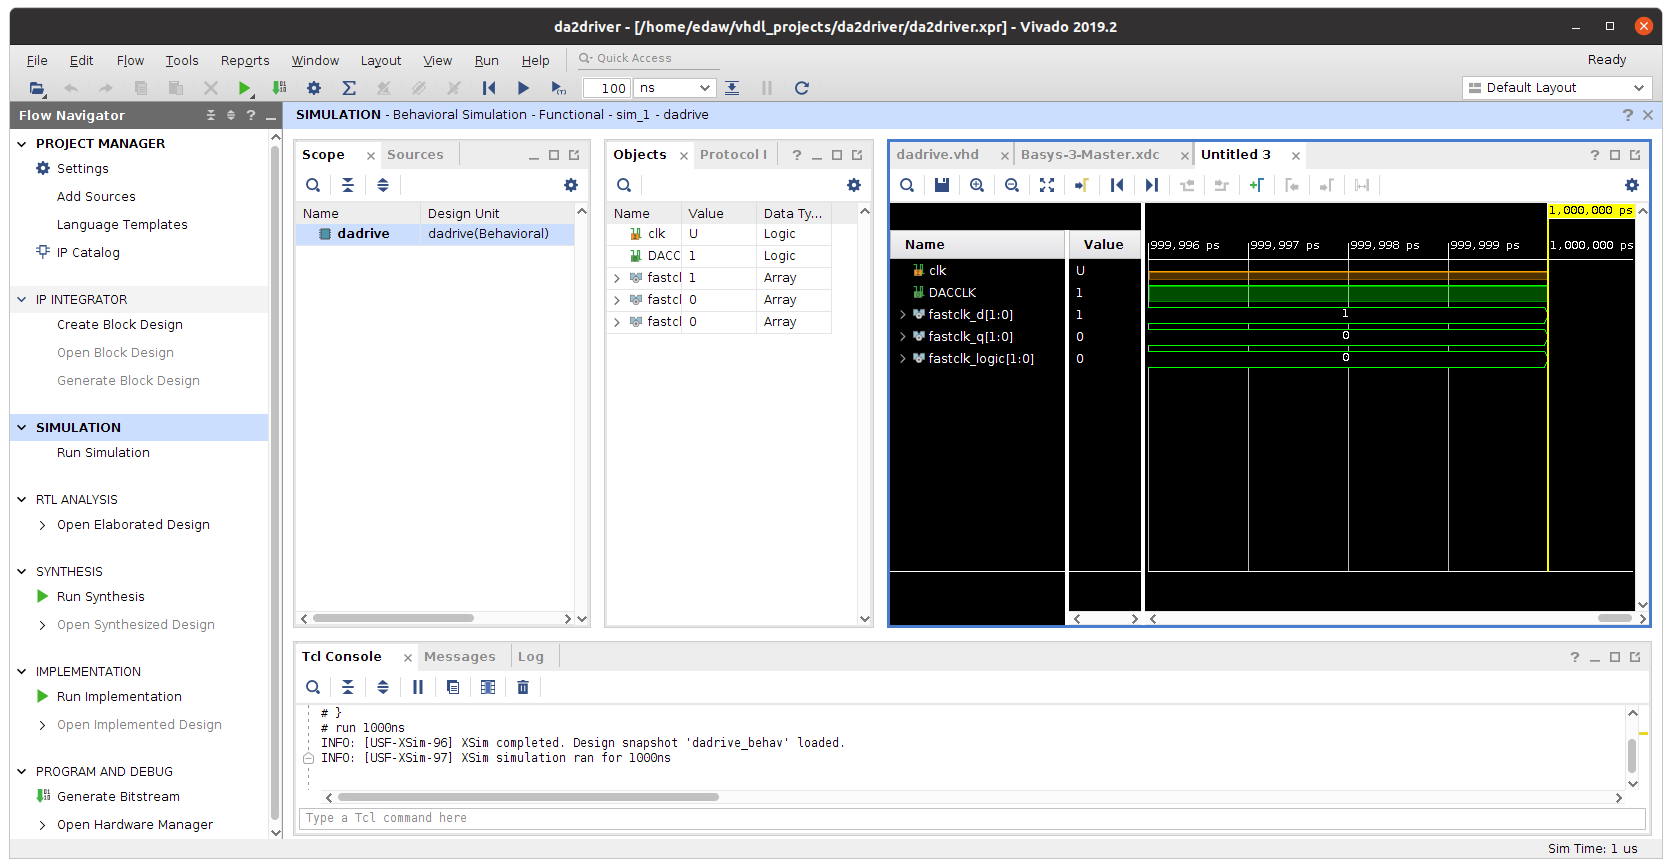
\includegraphics[width=1.0\textwidth]{appendix_7/figures/vivado_aftersimstart.png}
    \caption{The VIVADO screen after starting the simulation}
    \label{fig:vivdac1}
\end{figure}
\begin{figure}[htbp]
    \centering
    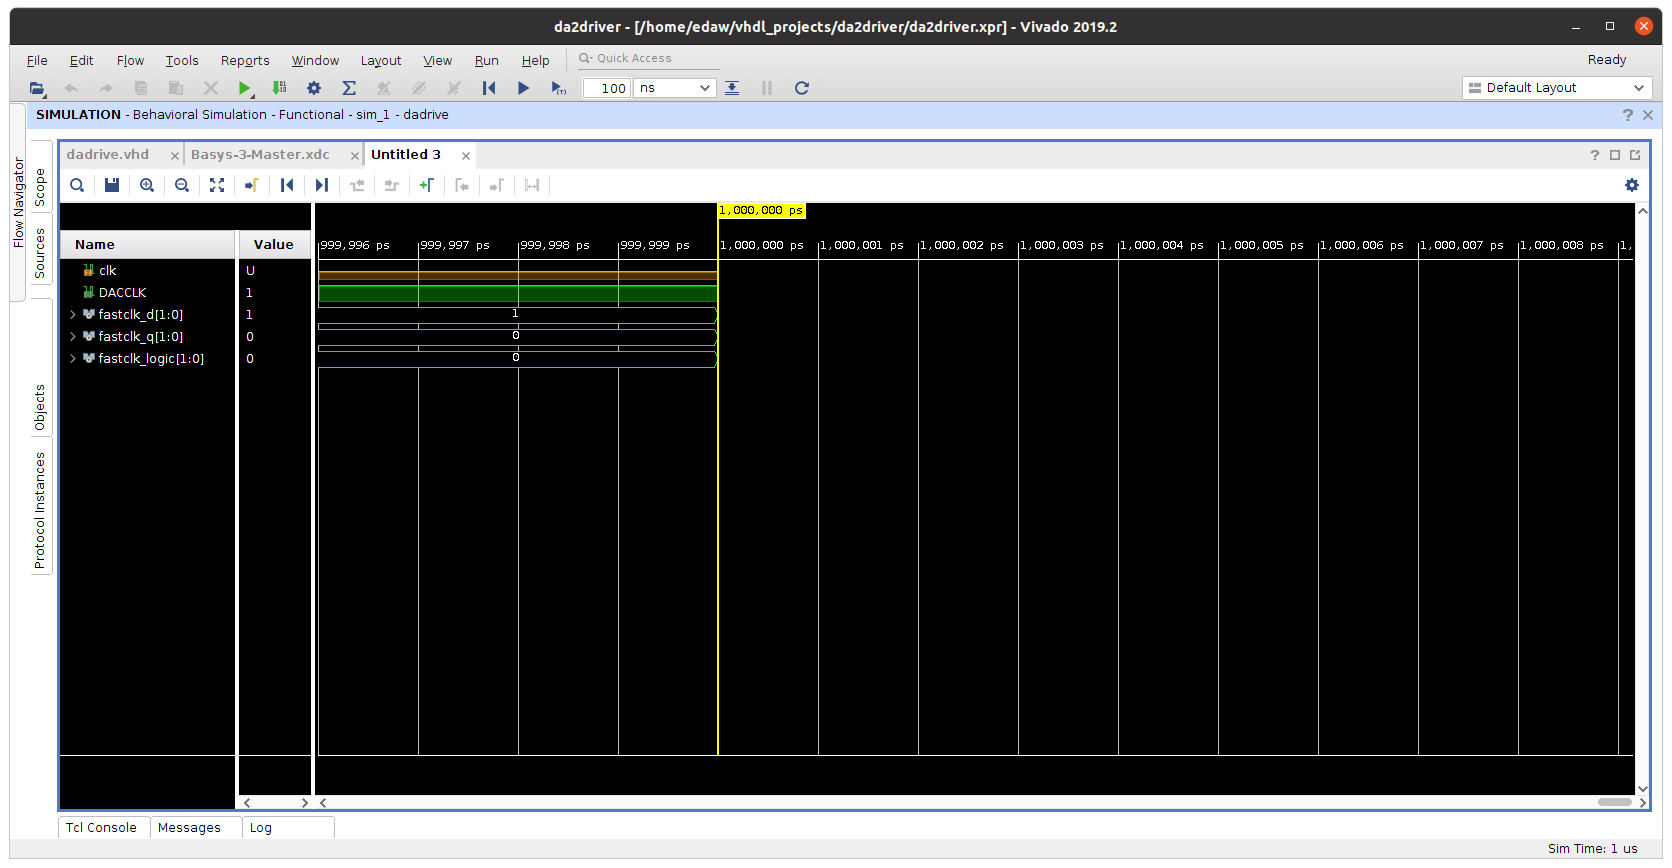
\includegraphics[width=1.0\textwidth]{appendix_7/figures/vivdac2.png}
    \caption{The VIVADO screen after minimising the other panes}
    \label{fig:vivdac2}
\end{figure}

The \texttt{clk} signal is orange because its state in the simulation is undefined. To set this signal as a 10ns clock, you right-click over the `clk' in the simulation and select `Force Clock'. In the window that appears, you set the Value radix as binary (this just tells the simulator that you want to display its value after simulation as binary), the leading edge and trailing edge signals to 1 and 0 respectively, leave the Starting time after offset at zero ns, leave the cancel box blank, leave the duty cycle at 50\%, and set the period of the clock to 10ns (matching the clk signal on the BASYS3 board). Then select OK. 

To run the simulation for, say, 200ns, go to the box in the middle of the top of the Vivado window, where the time $\rm 100\,ns$ is the default, and change to 200, leaving the $\rm ns$ as it is. Now, immediately to the left of the 200, there is a small arrow to th eright with a (T) under it. This is a timed simulation. Click on this arrow once. The simulator output should resemble Figure \ref{fig:vivdac3}. It doesn't look very interesting because the display shows only the last 10ps of the simulation. You will need to zoom out using the magnifying glass with a minus sign icon in the top left of the simulation pane. You can also use the horizontal scroll bar below the simulation output pane to position the piece of the simulation you are interested in appropriately. Note that the simulation tool by default does nothing until 1000\,ns, displayed as \texttt{1,000,000\;ps}, so if you only ran the simulation once the time period you are interested in is between \texttt{1,000,000\;ps} and \texttt{1,200,000\;ps}. Click on the $>$ to the left of the signal for the output of the clock storage register so you can see the display of the binary bits of the clock as well as the decimal value.

\begin{figure}[htbp]
    \centering
    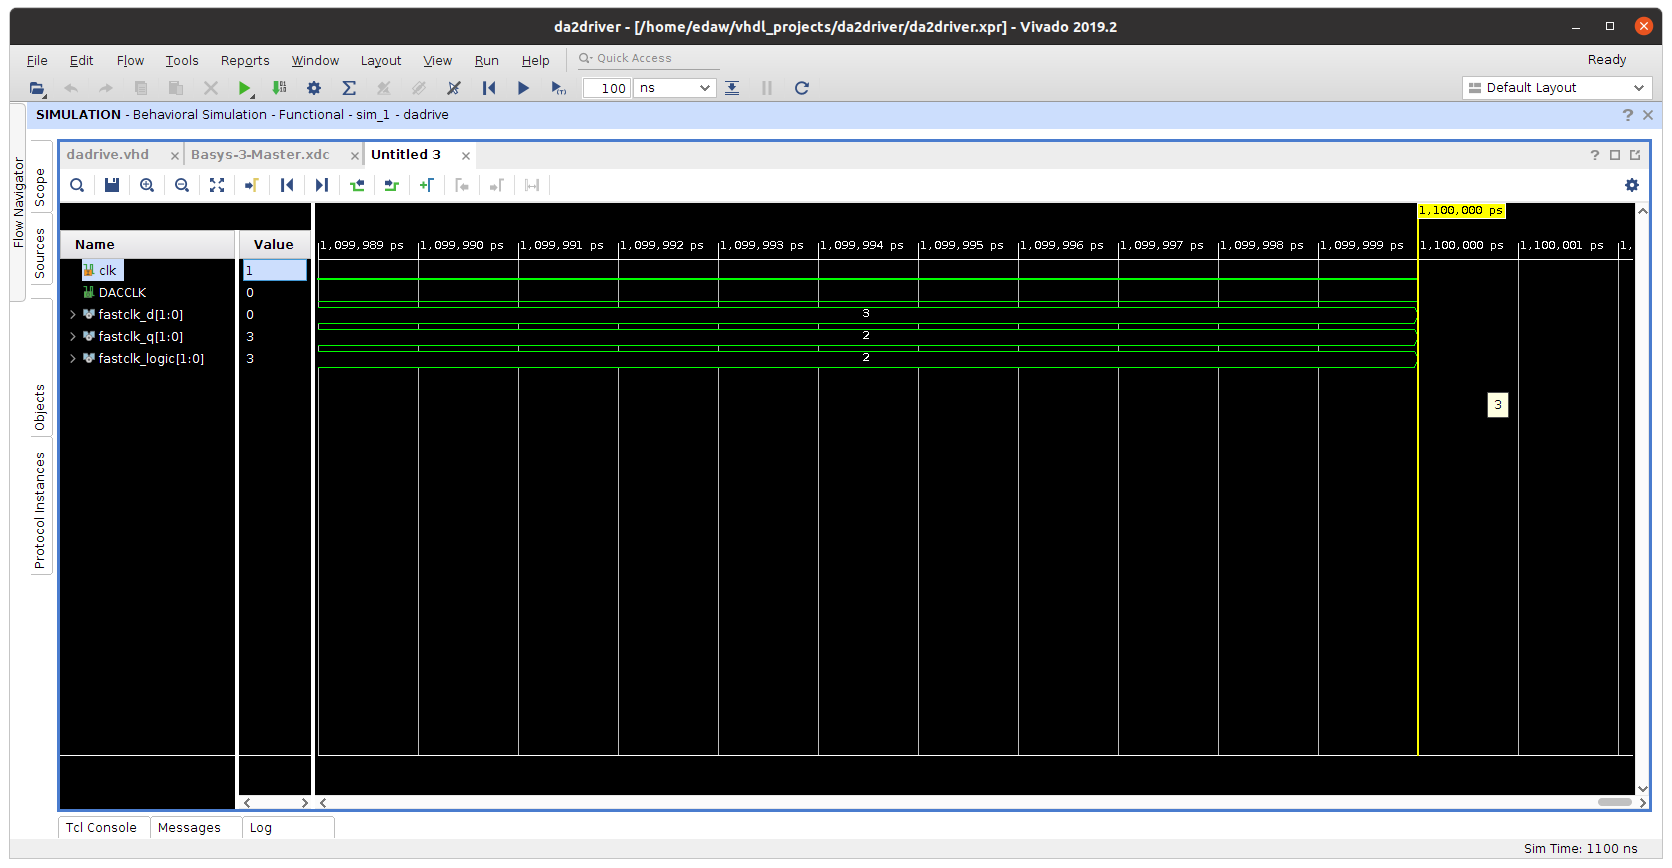
\includegraphics[width=0.8\textwidth]{appendix_7/figures/vivdac3.png}
    \caption{Simulation results before rescaling}
    \label{fig:vivdac3}
\end{figure}
\begin{figure}[htbp]
    \centering
    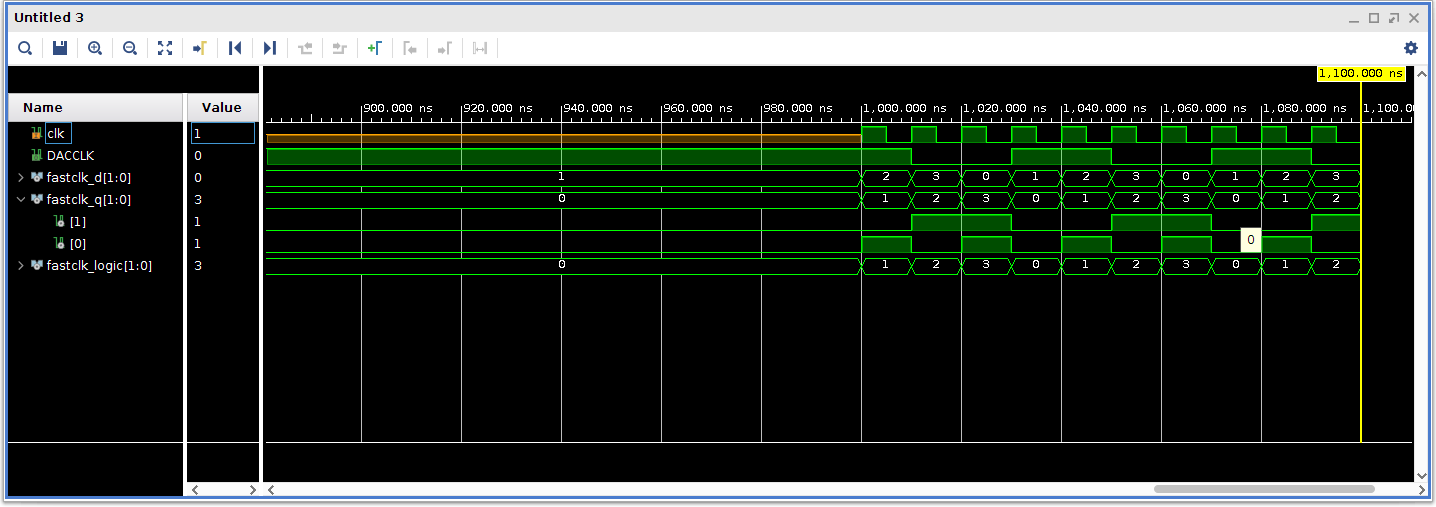
\includegraphics[width=0.8\textwidth]{appendix_7/figures/vivdac4.png}
    \caption{Simulation results after rescaling}
    \label{fig:vivdac4}
\end{figure}

Notice in the simulation results that the DACCLK signal is in antiphase with the most significant bit of the `Q' output of the clock register, in my simulation called
\texttt{fastclk\_q}. Notice also that the falling edge of the DACCLK signal, which will
be the signal to the PModDAC2 board to read the next data bit, occurs when the 
\texttt{fastclk\_q} signal is transitioning between 1 and 2. If everything looks right, close the simulator. If things don't look right, try and figure out what you haven't done right in
your VHDL code, or ask for help. Note that if you alter your VHDL code and want to re-simulate, you'll need to close the simulation using the blue cross in the top right hand
corner, and re-start it again.

\section{Slow clock and alignment}
\label{sec:slowclk}

We have a total of 16 bits of data to send, and we also need to rest the DAC chips by
setting $\rm \overline{SYNC}$ to high for a single period. Therefore we need a slow
clock that counts from 0 to 16 and then resets and does it all over again. Because
this is 17 cycles, we cannot use the natural overflow of a binary counter to do the 
reset, and we will have to do it using a conditional assignment.

Figure out how many bits a binary counter needs to be able to hold the numbers 0 to
16 inclusive, and create a slow clock buffer that turns over when the fast clock
transitions from 3 to 0. It should reset to 0 after it reaches 16. See if you can 
figure out how to code this up in your project. Don't forget to initialise your new registers to zero in the signal statement and include the appropriate register signal in the sensitivity list for the clk edge process. Don't forget that if you use a conditional assignment for setting the next value of the slow counter, Then, re-simulate and see if your simulation output looks like that in Figure \ref{fig:vivdac5}.

\begin{figure}[htbp]
    \centering
    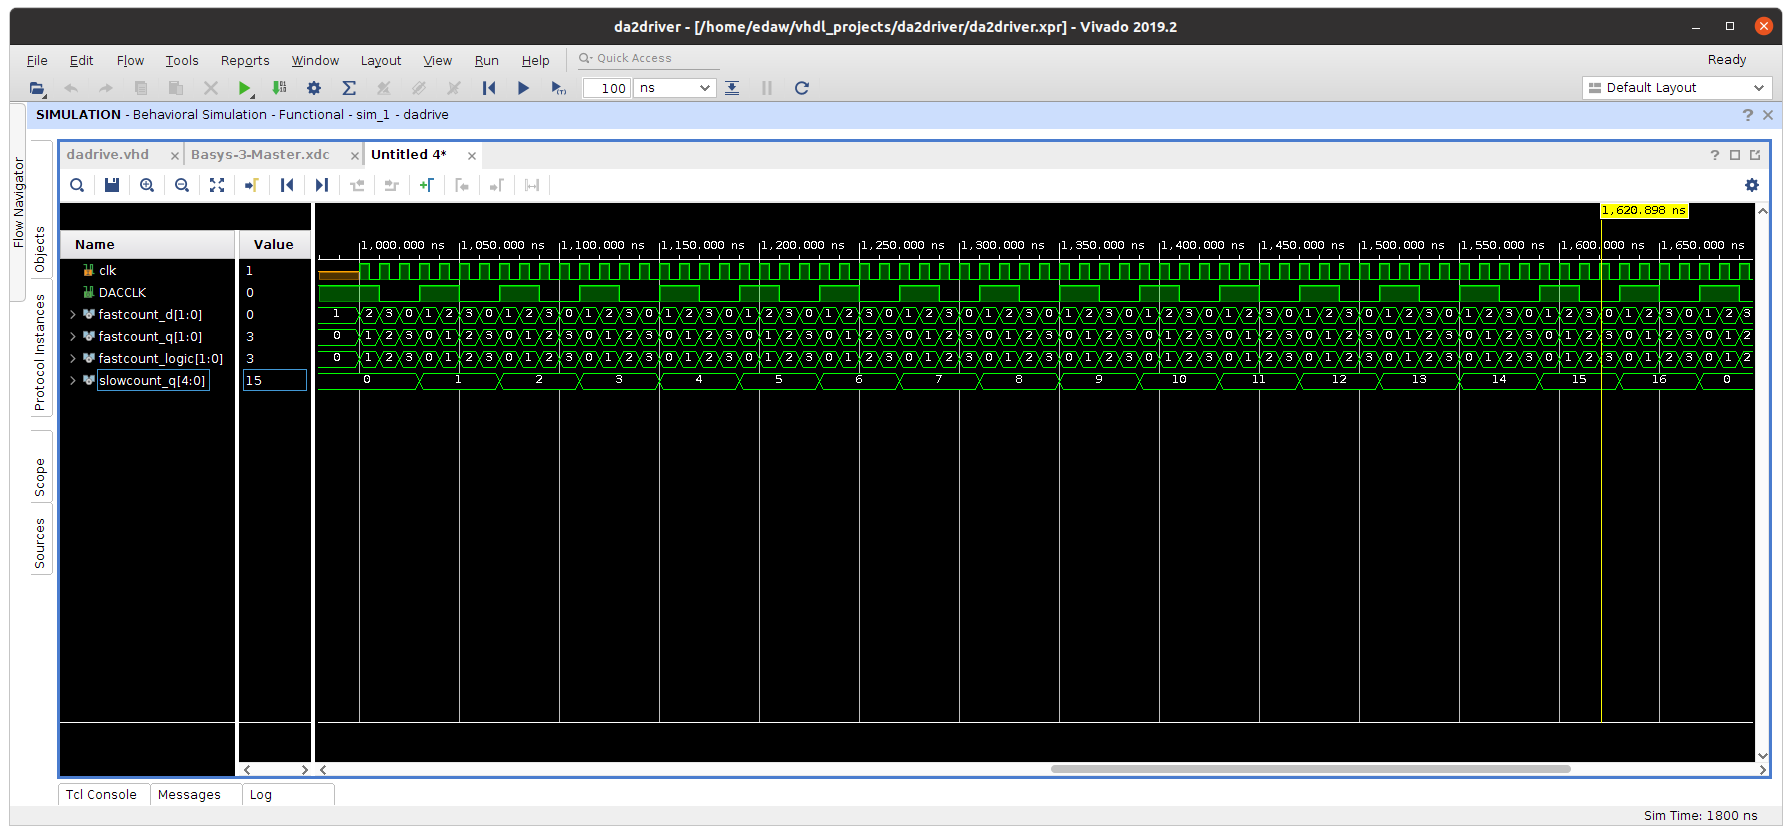
\includegraphics[width=1.0\textwidth]{appendix_7/figures/vivdac5.png}
    \caption{Simulation results with the slow counter added}
    \label{fig:vivdac5}
\end{figure}

Notice that the falling edges of the DACCLK signal occur half way thorough the cycles of the slow counter, and that the slow counter counts from 0 to 16 inclusive then resets. Check that your simulation output has this behaviour and ask for help / debug it yourself if it does not.

\section{Enable signal}
\label{sec:enable}

Next is the $\rm \overline{SYNC}$ signal. This signal should be high when the slow counter is zero and low otherwise. Implement this in VHDL and check with the simulation.

\section{A ramp waveform generator}
\label{sec:databuffer}

A ramp waveform rises linearly from zero to a maximum voltage, then resets quickly to 
zero, and the cycle repeats. If we drive our DAC with a counter, then we can make a ramp generator. The DAC has 12 bits, so there are $2^{12}$ or 4096 counts to go from all 12 bits zero to all 12 bit ones. If you want the ramp to have a period of 1 second, then the count must increment roughly every 1/4096 seconds or $\rm 0.24\,ms$. This is about 24,400 $\rm 10\,ns$ clock cycles. So, one way of making the ramp of roughly the right period is to have another fast counter with the right number of bits to reset roughly every 24,400 clock cycles. The required number of bits is $\log_2(24400)=\log_{10}(24400)/\log_{10}(2)\sim15$ bits. Therefore add to the code a
counter with 15 bits that is incremented every cycle. Also create a 12 bit data buffer, again using an unsigned data type, and increment this data buffer by 1 only when the 15 bit counter is zero. This way, the 12 bit counter should contain a digitised 12 bit ramp waveform with a period of order one second. 

Create two external ports, called \texttt{DATA1} and \texttt{DATA2}. Wire 
\texttt{DATA2} permanently to '0' as we are not going to use it. \texttt{DATA1} will
be the serial port output of our ramp generator. Refer to the PmodDA2 reference 
guide under `Interfacing with the Pmod' for the contents of the 16 successive 
bits read. The bits are fed in from MSB first to LSB last.

Therefore, \texttt{DATA1} must be 0 when the slow counter register output is less than or equal to 4 (when the slow counter register is zero, that's when the SYNC signal is high; when it's between 1 and 4 inclusive, that's when the unused 4 bits of data are expected at the DAC. On slow counter values 5 to 15 inclusive, bits
11 to 0 of the databuffer register output should be connected to \texttt{DATA1}. So
the number of the bit you are sending is 16 minus the value of the counter, for
counter values starting at 5 and ending at 16. A 
convenient way of writing the code would be to use the value of the counter itself
to index the array of bits making up the data buffer.

Using a logic vector value as an index for an array is not something we have covered yet in VHDL. This is the mechanism. The value of the counter is cast using \texttt{to\_integer}. VHDL presumably chooses an appropriate bit width for the 
hardware to select which bit. The syntax is shown below in the code listing.
The code listing assumes that the buffer containing the data is called
\texttt{datacounter\_q}, and the buffer containing slow counter is called
\texttt{slowcount\_q}. You will also need a signal with 12 bits that is a 
cast to \texttt{std\_logic\_vector} of \texttt{databuffer\_q}, so that you can
extract single bits from the data. Don't forget that bitwise operations in VHDL
only work on logic or logic vector data tyles. Let's call the 12 bit wide
\texttt{std\_logic\_vector} signal \texttt{datalogic}

\begin{minted}{vhdl}
-- cast contents of databuffer_q to a signal for a logic vector 
-- of the same length.
datalogic <= (std_logic_vector)databuffer_q;
-- slowcount_q has 5 bits and you are trying to set it to 5, hence
-- two 5s. The second line contains the array indexing. You could
-- also use a huge conditional assignment and deal with each
-- possibility for the slow counter separately. This is more typing,
-- but just as efficient code-wise.
DATA1 <= '0' when slowcount_q < to_unsigned(5,5) else
             datalogic(16-to_integer(slowcount_q));
\end{minted}

Once you think you have the \texttt{DATA1} output behaving correctly, and the 
ramp being generated with the right period in \texttt{datacounter\_q}, use the
simulator again to check its functionality. This time you'll need to simulate
for enough cycles so that the value of \texttt{databuffer\_q} has a chance
to increment a few times. Once it gets a value far from zero, you'll be able to
examine the value of the bits appearing serially in \texttt{DATA1} to see if 
the stream of bits matches the value of the databuffer. So, for example, if
databuffer was \texttt{0x3a} then this is $3\times 16+10=58$. In binary this
is $B000000111010$ which is $2+8+16+32=58$. I ran a long simulation (just adjust
the simulation duration to something like 20ms) then zoom out on the far end
(right hand end) of the simulation, and click somewhere in the window. A vertical
yellow line appears. Now use the magnify-+ button to zoom in on the neighbourhood
of that line. Note the value of the data buffer, and then see if the bit pattern
in DATA1 matches up. In Figure \ref{fig:simlong} I have shown my simulation at around 
$\rm 18.95\,ms$ after the start.

\begin{figure}[htbp]
    \centering
    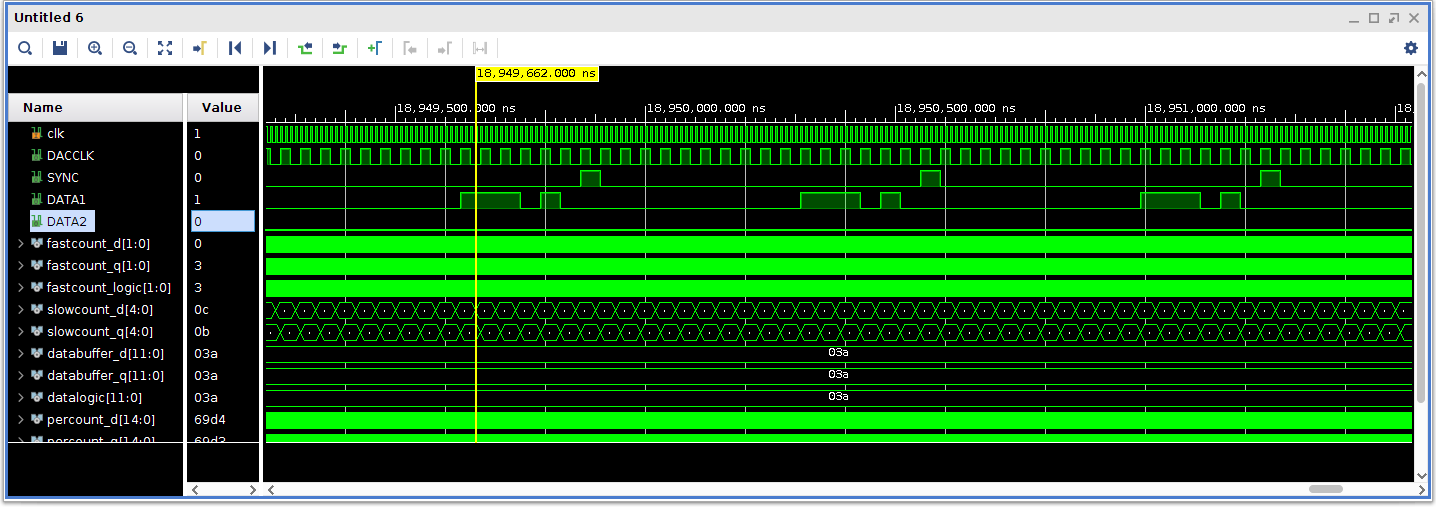
\includegraphics[width=1.0\textwidth]{appendix_7/figures/simlong.png}
    \caption{Simulation results showing the serial port. You can see that
    the value stored in datalogic is \texttt{0x03a}, which as
    hexadecimal for 58. The value in \texttt{DATA1} has its least 
    significant bit just before the SYNC line goes high. The first
    few bits from LSB to MSB are $0,1,0,1,1,1,0,0$ and the rest of the
    bits are zero. This indeed corresponds to decimal 58, so this
    appears to be working.}
    \label{fig:simlong}
\end{figure}

\section{Connecting up the PMOD chip}
\label{sec:connections}

If you are at home, you won't easily be able to check that the hardware
connected to the PMOD port actually works as advertised. However, there is
one way you can do this - if you reduce the number of bits in the ramp
generator counter from 15 bits to 6 bits, then an earphone connected between pin 1
(analog output 1) and pin 5 (ground) on the output of the PMOD card connected
to the BASYS3 (you can just plug it in then build and deploy the code
if the simulator predicts it will work correctly), will make an audible tone.

For a more challenging readout, use 15 ramp generator counter bits, not 
six as for the earpiece output. You can then import the ADC from last weeks 
project, wire it up to the LEDs, and connect two cables, one between 
the PmodDA2 ground and the inverting input to channel 2 of the XADC 
input, and the other between the PmodDA2 analog output 1 (pin 1) and the
non-inverting input to channel 2 of the XADC. You can then internally 
connect the digital output from XADC to the LEDs and watch them light 
up to represent the ramp signal as it evolves.

Finally, if you are in the lab, you can connect an oscilloscope probe between
pin 1 and pin 5 on the PModDA2 output connector, and see if you can record the 
ramp on an oscilloscope trace. If you are going to do this, you might want to
reduce the number of bits for the counter to 6 so that the ramp period is 
less than 1/100 of a second, as the oscilloscope will be easier to handle
if the waveform is faster.

\end{document}